\documentclass[manuscript,screen,nonacm,12pt]{acmart}
%% NOTE that a single column version is required for 
%% submission and peer review. This can be done by changing
%% the \doucmentclass[...]{acmart} in this template to 
%% \documentclass[manuscript,screen,review]{acmart}
%% 
%% To ensure 100% compatibility, please check the white list of
%% approved LaTeX packages to be used with the Master Article Template at
%% https://www.acm.org/publications/taps/whitelist-of-latex-packages 
%% before creating your document. The white list page provides 
%% information on how to submit additional LaTeX packages for 
%% review and adoption.
%% Fonts used in the template cannot be substituted; margin 
%% adjustments are not allowed.
%%
%% \BibTeX command to typeset BibTeX logo in the docs
\AtBeginDocument{%
  \providecommand\BibTeX{{%
    \normalfont B\kern-0.5em{\scshape i\kern-0.25em b}\kern-0.8em\TeX}}}

    \addtolength{\baselineskip}{4pt}
%% Rights management information.  This information is sent to you
%% when you complete the rights form.  These commands have SAMPLE
%% values in them; it is your responsibility as an author to replace
%% the commands and values with those provided to you when you
%% complete the rights form.
\setcopyright{acmcopyright}
\copyrightyear{2018}
\acmYear{2018}
\acmDOI{10.1145/1122445.1122456}
 

%%
%% These commands are for a JOURNAL article.
\acmJournal{POMACS}
\acmVolume{37}
\acmNumber{4}
\acmArticle{0}
\acmMonth{8}

%%
%% Submission ID.
%% Use this when submitting an article to a sponsored event. You'll
%% receive a unique submission ID from the organizers
%% of the event, and this ID should be used as the parameter to this command.
%%\acmSubmissionID{123-A56-BU3}

%%
%% The majority of ACM publications use numbered citations and
%% references.  The command \citestyle{authoryear} switches to the
%% "author year" style.
%%
%% If you are preparing content for an event
%% sponsored by ACM SIGGRAPH, you must use the "author year" style of
%% citations and references.
%% Uncommenting
%% the next command will enable that style.
%%\citestyle{acmauthoryear}

%%
%% end of the preamble, start of the body of the document source.
\begin{document}

%%
%% The "title" command has an optional parameter,
%% allowing the author to define a "short title" to be used in page headers.
\title{Design and Co-design of Learning Analytics Dashboards}

%%
%% The "author" command and its associated commands are used to define
%% the authors and their affiliations.
%% Of note is the shared affiliation of the first two authors, and the
%% "authornote" and "authornotemark" commands
%% used to denote shared contribution to the research.


%%
%% By default, the full list of authors will be used in the page
%% headers. Often, this list is too long, and will overlap
%% other information printed in the page headers. This command allows
%% the author to define a more concise list
%% of authors' names for this purpose.
\renewcommand{\shortauthors}{Author, et al.}

%%
%% The abstract is a short summary of the work to be presented in the
%% article.
\begin{abstract}
  Co-Design of LAD
\end{abstract}
%\ccsdesc[500]{Computer systems organization~Embedded systems}
%\ccsdesc[300]{Computer systems organization~Redundancy}
%\ccsdesc{Computer systems organization~Robotics}
%\ccsdesc[100]{Networks~Network reliability}

%%
%% Keywords. The author(s) should pick words that accurately describe
%% the work being presented. Separate the keywords with commas.
\keywords{learning analytics, learning analytics dashboard, participatory design, co-design}


%%
%% This command processes the author and affiliation and title
%% information and builds the first part of the formatted document.
\maketitle

\section{Introduction} 
Learning analytics dashboards are designed to use learners' traces to present the computed indicators and other visual elements in a clear and intuitive way \citep{Brouns2015}.
They have emerged as applications for visualizing and interacting with data collected in a learning environment in various forms \citep{Ramos2015}. \citet{Steiner2014} referred to them as ``visualizations of learning traces''. For \citet{Yoo2015}, a learning dashboard is ``a display which visualizes the results of educational data mining in a useful way''. 
\citet{Schwendimann2017} identified a lack of an agreed and shared definition and thus proposed the following:
\begin{quotation}
	``\textit{%
		A learning dashboard is a single display that aggregates different indicators
		about learner(s), learning process(es) and/or learning context(s) into one or
		multiple visualizations.
	}'' \citep{Schwendimann2017}
\end{quotation}
Learning dashboards provide interactive, historical, customized and analytical displays that are based on the results of  analyzing learning data \citep{Park2015, Kim2015}. By implementing visual and interactive analytics, they amplify human natural abilities to detect patterns, establish connections and make inferences. The produced visual outputs can significantly highlight aspects of interest from the mined and discovered knowledge~\citep{Duval2011}. According to \citet{bennett2019four}, we can distinguish  three types of learner dashboards: predictive, modeler and descriptive. 
\begin{itemize}
    \item Predictive types use machine learning based on computer algorithms that rely on a series of trace data to predict the likelihood that the students outcomes. Many works in this category (i.e, \citep{arnold2014exercise}) use these algorithms to produce at risk rating for individual students.
    \item For example, aspects of a student's online behaviors such as communication, initiative, presence that have been derived from the number of messages, the number of comments in response to others' messages, time spent online, etc., are not included in this section. 
    \item The third type of dashboard is descriptive and displays past learning behaviors
\end{itemize}


Learning dashboards are suitable for online,  face-to-face, and blended learning \citep{Verbert2013}. They can target different stakeholders: administrators, instructors, learners or all of them. 
Within a single display, indicators and visualizations about learners, learning processes and contexts are rendered using different shapes, from plain text to visual elements (e.g., tables, spreadsheet charts, scatterplot, 3D representations) to complex artifacts such as alerts and notifications that prompt interventions~\citep{Few2006, Podgorelec2011, Schwendimann2017}. 
Currently, they are increasingly deployed as a meaningful component in learning analysis systems. For instance, they are currently used in studying progression through courses \citep{Nicholson2012}, learners level of attainment~\citep{Gutierrez2012}, and learners' engagement from the cognitive and behavioral perspectives \citep{carrillo2017dashboard}.
Despite being fairly recent educational tools, the research found many benefits of using learning dashboards to improve learning performance \citep{Arnold2012} and to increase learners' motivation  \citep{Verbert2013, Wise2016}.


\section{Issues in current LA design approaches}
The design and evaluation of learning dashboards is a major area of inquiry in learning analytics research.
There is a growing body of literature on learner dashboard design. A comprehensive literature review by \citet{bodily2017trends} involved identifying and analyzing 93 papers with respect to functionality, data sources, design analysis, student perceptions, and measured effects. They found that the clear majority of the papers focused on technical features such as data sources, functional aspects (e.g., visualization data, what the dashboard was intended to do) while only two papers reported on how students' behaviors were changed as a result of using the Learner Dashboards and only one-third (34 of 93) focused on students' perceptions of the design.
\subsection{General design principles}
Due to the recent emergence of learning analytics dashboards, there is still a scarcity of studies on their design principles \citep{Echeverria2018}. 
\citet{Yoo2015} argued that, since dashboards are an instrument of communication, effective design is tied to several theoretical foundations, such as human cognition and perception, situational awareness and visualization technologies. In other words, their conceptualization must be based on an understanding of how humans see and think. 

Based on a number of theoretical principles in addition to his practical experience, \citet{Few2013} outlined some good and bad examples of dashboard design. He claimed that the essential characteristics of a dashboard are: 
1) to be visual displays; 2) to display the information needed to achieve specific objectives, 3) to fit on a single computer screen, and 4) to be used to monitor information at a glance. 
In terms of human perception, due to the limited working memory of humans, only three or four pieces of visual information can be stored at a time.  Therefore, for more effective memory perception and retention, it is essential to incorporate graphic patterns such as graphs rather than individual numbers. In addition, there must be a proper and reasoned use of pre-attentive attributes such as colour, shape, spatial position and movement.
From Few's principles, \citet{Yoo2015} drew three main implications: 
\begin{enumerate}
	\item the most important information should stand out from the rest in a dashboard, which usually has limited space to fit into a single screen;
	\item the information in a dashboard should support one's situated awareness and help rapid perception using diverse visualization technologies; and
	\item the information should be deployed in a way that makes sense, and elements of information should support viewers' immediate goal and end goal for decision making.
\end{enumerate}

\textit{Situational awareness} deals with disclosing the type of information that is important for a particular purpose or task \citep{Endsley2016}, and thus constitutes another design principle related to dashboards. Three levels can be distinguished:
\begin{enumerate}
	\item perception of the elements in the environment;
	\item comprehension of the current situation; and
	\item projection of future status.
\end{enumerate}
\textit{Situational awareness} is commonly understood in terms of people being consistently aware of what is going on, in order to predict what will be happening as well as to prepare what must be done. 



\subsection{Limitation of the current  design approaches}
%TODO: COPY/PASTE from etd9277_SShiraziBeheshtiha.pdf

%Echeverria2018
\subsubsection{Lack of theoretically informed design}
%The majority of educational dashboards are based on theories and practices related to information and data visualization. 
\citet{alhadad2018visualizing} noted that data visualization design should be grounded in theories of cognitive learning. Yet, many authors reported  the absence of design choice justifications in the conception of several learning dashboards \citet{Bodily2017}. For example, attention to issues of cognitive loading, attention, human perception and data literacy has direct design implications, such as avoiding visual clutter and breaking down data into segments that can be interpreted on the screen. This perspective is consistent with what data visualization researchers understand to be visual coding and interaction design decisions \citep{munzner2014visualization}, where choices regarding graphic types, interface components such as text and placement of visual markers, and interactive elements align with what is known about cognition and perception.


%Sometimes, to represent the analyzed data from different angles, designers use complex representations and visualizations that are rather difficult for end users to interpret, especially "at a glance" \citep{Duval2011}. 


A primary concern of dashboard designers must be the identification of what type of visual representations to implement, and what kind of interaction to offer. Indeed, one obstacle to the adoption of dashboards is the often existing gap between visual analyses and the objectives of the study  \citep{Roberts2017}. This is shown in the survey reported by \citep{Reimers2015} where the existing dashboards generally were found to have poor interface design and lack of usability testing. 
\citet{Gavsevic2015} argue that, without careful considerations, the design of dashboards can result in the implementation of fragile and undesirable instructional practices by promoting ineffective feedback types and methods. 
In order to encourage adoption of learning dashboards, the design needs to be further informed by theories related to learning sciences and educational psychology. 


\subsubsection{Selection of the input data and the computed indicators}
A rich variety of measured data and indicators are used and computed in existing dashboards. 
Dashboard solutions are heavily based on trace analysis, and little attention has been paid to use other data sources such as direct feedback or the quality of the produced artifacts.
Moreover, as noted by \citet{Schwendimann2017}, there is little work on comparing which indicators and which visualizations are most suitable for the different user data literacy levels.
In most cases, the chosen visualizations are rather similar to those in other areas of dashboard applications (e.g., web analytics),
which highlights the lack of specific visualizations and visual metaphors that address the activities of learning and teaching (another potential area for future research) \citep{Schwendimann2017}.

\subsubsection{Learners' aptitudes are not considered}
The review of \citet{Schwendimann2017} revealed that current focus hugely falls on the information that can be extracted from the log data rather than how individual differences might affect the interpretation of the information presented to the learner in terms of reflection and taking actions \citep{Gavsevic2015}. 

%here :
Studies undertaken by \citet*{bodily2017trends}  and \citet*{viberg2018current}  also point to  the need to understand users' views of dashboards qualitatively and in use rather than  as technical artefacts. This conception foregrounds the purpose of the tool in that it considers how  students make use of information presented via the dashboard and how it might change their  behavior as a result. Dashboard conception needs also to focus attention on the perspective of  the user, the learner, and on the purpose of dashboards as tools that provide feedback to students  to encourage them to make more informed decisions about their study behaviors \citet*{howell2018learning,bennett2019four}.

\subsection{Need to involve dashboard stakeholder in the design process}

While the primary purpose of LA tools is to promote learning, there is a risk that these tools impose a number of assumptions that do not necessarily meet the students' or educators' needs \cite{dawson2015challenging}. One main reason identified by many authors (e.g. \cite{buckingham2019human}) is the lack of active stakeholder collaboration in the process of design of these tools. 
For instance, the selection of data to be visualized is generally not what the stakeholders in the analysis want or really need because they have not regularly been involved in the design process \citep{Holstein2017}.
These authors suggest that including end-users in the design process ensures appropriate design responses that are aligned with end-user requirements \cite{taffe2015hybrid}. 

According to \citet{beattie2014creepy}, failure to involve learners and educators in the decision-making process can hinder the adoption and acceptance of LA innovations. \citet{Holstein2017} also argued that the success of the dashboards depends greatly on the degree to which its stakeholders have been involved in co-designing them. 

\section{Co-design of learning analytics dashboard}
The goal of designing data visualizations is to empower users to better understand the data presented by the visualization, so the user must be kept in mind when designing data visualizations. 
To glean as much information as possible about the context and needs of users, 
a common strategy is to use participatory design techniques where end-users are directly invited to participate in the design process. 

\subsection{Designing with users of software systems}
Service design process is human-centered since it is based on the assumption that a design object has no significant meaning unless it becomes part of the lived experience of people \cite{krippendorff2005semantic}.
Capturing users' unique knowledge about usage and latent needs during this process  is key to innovation and new service success \cite{mahr2014value}
Two concepts are relevant in this context: human-centered design and user-centered design :
\begin{itemize}
    \item \textit{Human-centered design} (and \textit{User-design}) focuses on creating systems that are easier to use by taking human factors into account.
    \item \textit{User-centered design} involves users in the design process where design development is influenced by end-users. Model-based, story-based and scenario-based design are examples of user-centered design methodologies. 
\end{itemize}

According to \citet{ivanov1995subsystem}, there is a very significant differentiation between \textit{user-design} and \textit{user-centered design} in that user-centered design is a useful and important construct, but one that suggests that users are taken as centers in the design process, consulting strongly with users, but not allowing them to make decisions or giving them the tools that experts use. 

For \citet{vilpola2008method}, user-centered design is an an imperative part of creating products that ensures usefulness to users, and that allows creation of systems that fulfill users requirements. The authors highlight four principles of user-centered design: (1) user is actively involved; (2) user's tasks and technological function must be distinguished; (3) the design should be iterative; and (4) the design should be multidisciplinary. 
\citet{vredenberg2001user}, while recognizing that user-centered design improves product usefulness and usability, pointed out a lack of effectiveness measures to evaluate the success of a user-centered design effort.

\subsubsection{Participatory design}
\textit{Participatory design} and \textit{Co-design} derived from user-centered design as a particular case of co-creation where designers who are trained in creativity work together with non-designers during the design process. 
In  software development, \textit{participatory design} can be thought of as a movement from end-users to the world of researchers and developers, while \textit{empathic design} is much more seen as a movement from researchers and developers to the world of end-users. Its main purpose is to empower participants to become legitimate and acknowledged members of the design team \cite{visser2005contextmapping}.
\citeauthor{prahalad2004future} are usually given credit for bringing co-creation/co-design to the minds of those in the business community with the 2004 publication of their book "{The Future of Competition: Co-Creating Unique Value with Customers}". According to the authors: \textit{
"The meaning of value and the process of value creation are rapidly shifting from a product and firm-centric view to personalized consumer experiences. Informed, networked, empowered and active consumers are increasingly co-creating value with the firm."} \cite{prahalad2004future}

Often participatory design is referred to in discussions of user-centered design, so the difference between user-centered design and participatory design has become quite unclear \cite{bannon2018introduction}. Yet, participatory design is sometimes discussed alongside user-centered design, as a user-centered approach \cite{leng2018designing}.
On the other hand, the terms \textit{Participatory design} and \textit{co-design} are often used  interchangeably. Yet, Some authors make the distinction by stating that the term co-design has come more recently to denote a specific type of participatory design. For instance, \citet{szebeko2010co} state that "Co-design differs from some of these areas as it includes all stakeholders of an issue not just the users, throughout the entire process from research to implementation." For \citet{Sanders2008} "the terminology used until the recent obsession with what is now called co-creation/co-design" was "participatory design".

The emergence of participatory design, according to \citet{bannon2018introduction}, was motivated by the need to involve users in the process of design, and to help mitigate situations of divergent ideas through democratic decision-making processes. 
For \citet{dearnley1983favour}, participation in design emerged: firstly, as a means of mitigating the problem of conventional approaches that do not work; and secondly, because of ethical issues, claiming that end-users should have some influence over the environment in which they work.

Arguing that the design paradigm of participatory design is constructivism,\citet{spinuzzi2005methodology} assumes that knowledge exists in a certain context, not just in a person's mind. The author identified three stages of participatory design research: initial exploration of work, discovery processes and prototyping. 
\begin{itemize}
    \item \textit{Initial exploration of work}: this is the stage where users and designers meet to become familiar with how users work with each other. The used research methods are ethnographics and include observations, interviews and visits to the organization.
    \item \textit{Discovery processes}: during this stage, the design stakeholders use different techniques to improve their understanding, prioritize the organization of work, and construct a future vision for the workplace. The used methods include organizational games, role-play games, organizational toolkits, future workshops, storyboarding, and workflow models and interpretation sessions.
    \item \textit{Prototyping}: Here, users and designers form technological artifacts in an iterative manner, to fit into the future vision created in the second stage. This is achieved using different methods including mock-ups, paper prototyping, and cooperative prototyping.
\end{itemize}


\subsection{Participatory Design for Learning}
\subsubsection{Emergence of co-design in LAD}
In education, policy-makers typically rely on teams of visual designers, business specialists, and educational theorists who produce educational innovations. 
In the current literature on learning analytics, there are calls for theory-based and participatory approaches. Participatory design allows the involvement of the users of the system in the design process and gives stakeholders the opportunity to learn more about other stakeholders' views \cite{unger2013designing}. It is a process where designers and non-designers work together creatively ideally in all stages of design 
\cite{Sanders2008}. 

Within the learning analytics community, designers and researchers are increasingly turning to human-centered design methods to adopt practical design techniques and knowledge to explore the design cycle of a learning analysis project. 
However, as noted by \citet{dollinger2018co}, learning analytics researchers often work in applied contexts with real educators and educational settings, where it quickly becomes apparent that interface-level design decisions alone are not sufficient to productively promote effective use of visual dashboards. 


\subsubsection{Benefits of co-designing LADs}
Co-design is a collaborative, structured process with stakeholders explored over many years in software development, from initial implementation using participatory design (PD) techniques to the introduction of the concept into the LA \cite{prieto2020engaging}.
A main claim of co-design is that it remedies design’s conventional exclusion of people from design outcomes that affect them \cite{taffe2015hybrid}. 

A dashboard design team should include education administrators, technology experts, data managers and, most importantly, learners. The benefits of co-designing a dashboard with the collaboration of multiple stakeholders with diverse perspectives are numerous. 
This ranges from as a better understanding of authentic teaching and learning needs and expectations, developing or adapting analytical tools appropriate to educational intentions, building trust among stakeholders, to developing effective strategies for responsibly using sensitive data \cite{beattie2014creepy}.

A co-design approach encourages multi-stakeholder alignment with the primary purpose and objective of the dashboard, ensures consistent implementation by anticipating potential barriers or difficulties to adoption, and increases innovation capacity and efficiency \cite{boscardin2018twelve}. It also promotes consensus building and sharing of mental models for key learner outcomes, as well as the appropriate interpretation and use of assessment data by multiple stakeholders. As pointed out by \citet{schuler1993participatory}, a co-design approach reflects a participatory design movement that emphasizes mutual learning, with users learning about the opportunities and constraints of the technology while designers learn about user practices and perspectives.


\subsection{Co-design methods and techniques}
Participatory Design for Learning is a growing field with its own history, philosophies, and body of techniques and methods \cite{disalvo2017participatory}. In practical terms, the LA researchers used a subset of techniques such as pre-interviewing end-users about 
their needs to derive design ideas \cite{xhakaj2016teachers}, employing practitioner-partners as informant designers who give feedback on 
designs \cite{fiorini2018application}, and engaging teachers throughout the prototyping process itself to create classroom analytics \cite{holstein2018classroom}.

Different methods and techniques are being used to apply participatory design. The most popular include brainstorming exercises, card sorting, group affinity diagraming, rapid paper prototyping, wireframe walkthroughs, preferences testing \cite{abel2013cross}. 

\subsubsection{Focus groups}
One of the main benefits of using focus group sessions as a co-design technique is their effectiveness in collecting ideas that can be used for improvement and in identifying popular opinions among learners.  They provide a collective view of the problem and concerns, as opposed to information gathered through simple surveys where closed-ended questions are usually asked, limiting the feedback that participants can provide. They are also much more flexible than surveys or scales because they allow questions, clarifications, and follow-up questions to be asked for vague or unexpected answers \cite{krueger2014focus}. 

This technique is mostly used for qualitative purposes with reports being descriptive to depict the meaning of the data as opposed to a simple overview. Three main approaches are generally used for the analysis of focus group sessions to générate a report that includes the final interpretation of group
statements: \textit{Classical content analysis}, \textit{Keywords-in-context}, and \textit{Discourse analysis} \cite{prieto2018co}.



\subsubsection{Collaborative personas}
Learning persona allows modeling and summarizing essential information about the people who are likely to be involved in the learning ecosystem. A learner persona is therefore a hypothetical learner who is representative of a certain number of potential learners, educators, etc.
According to \citet{zhang2016data}, personas must help answer three basic questions: \textit{what are the learner’s needs, what kinds of limitations do they have, and what are their expectations?}
In terms of co-design, people can be invited to build Persona profiles or create their own representations that can be merged later in different instances \cite{prieto2018co}.

\subsubsection{knowledge mapping}
This technique is commonly used to make visible how a group understands key ideas and their connections \cite{prieto2018co}. It encompasses different well-known methods like  mind maps, concept
maps, dialogue maps and argument maps. For instance, mind maps are word lists structured and organized as trees to represent an idea, concept, or plan, while concept maps are diagrams that use lines to organize and represent relationships between concepts \cite{carrillo2017dashboard} (see \cite{okada2008knowledge} for details). Maps made by participants with pens and large sheets of paper are participatory in that everyone can contribute.

\subsubsection{Card-based co-design}
Numerous map-based design tools are available, mainly to help creativity and user participation in design. According to \citet{roy2019card}, cards are semi-structured tools between blank Post-it notes and detailed instruction manuals; they provide a common basis for understanding and communication in a team and support creative combinations of information and ideas. They thus  provide convenient summaries of useful information and/or methods.

\subsubsection{Sketching and Prototyping}
Sketches and prototypes can be used to converge the results of collaborative efforts with stakeholders. This making process allows constructing visual representations, engaging co-designers beyond the ideation process. Prototyping allows participants to communicate in a non-traditional way, by inviting them to communicate their needs and expectations \cite{gaver1999design}.
Reflection and interpretation are the primary objectives in building the first prototype that helps all learners involved understand what they are looking for in visual representations \cite{luckin2013handbook}.

Sketch-in is a group activity in which learners use sketching to solve design problems together, generally in quick sessions using basic drawing materials (post-its, paper sheets and whiteboards) \cite{prieto2018co}. For instance, participants can test data visualizations, color combinations, interaction styles, and define the characteristics that match the intended use.

\subsection{Examples of the use of co-design in LAD}
\citet{ruiz2018participatory} described a participatory design method for generating interface prototypes. The method is comprised of
different techniq ues, each one oriented toward the obtainment of
artifacts which are input for the technique that continues the
process within the method. The method is composed of different techniques, each oriented towards obtaining artifacts that are introduced into the technique that continues the process within the method. It explores, extracts, and integrates the needs, mental models, and perspectives of classroom teachers, students, and educators. The method is implemented in the design of an interactive educational system, which allows the elaboration of sequences of activities through the DSML language.

Motivated by the fact that the LA community lacks co-design tools adapted to the specific needs of LA actors to effectively communicate and understand design elements, LA-DECK was proposed as a card-based co-design tool specifically adapted to LA \cite{Alvarez2020}. The tool features 8 suits of cards, grouped into three main themes: Context, Strategy, and Action (making a total of 40 colored cards). According to a pilot study, the tool  promotes productive co-design of high-level concepts, facilitate communication in a team, allows  combinations of information and ideas, and offers convenient summaries of useful information and design methods.


\section{Participatory Design of Learning Analytics Dashboards}
\subsection{Rationale and requirements}
\subsubsection{An iterative refinement process}
\label{sec:dimensions}
We have conducted an iterative process to develop our needs-capture method. First we carried out a study to assess needs based on questionnaires and semi-directive interviews, and then, after evaluating  the findings of this first study, we organized a participatory workshop with the stakeholders.


\paragraph{Phase 1: Questionnaires and interviews}
We carried out a study to assess the capture needs based on questionnaires and semi-directive interviews with stakeholders from 8 case studies out of the 13 identified by the Hubble project \cite{dabbebi2017towards}. 
The objective was to develop an explicit understanding of the users' context, tasks, needs and environments in order to enable the dynamic generation of dashboards. This study included a survey and semi-structured interviews.

We adopt the framework proposed by \citet{chatti2012reference}, which identifies four questions around the analysis of learning data. We supplement theses questions with a fifthone, "When", which we felt was important for participants to better understand their interactions with learning dashboards. We thus list five questions where each refers to a contextual dimension "Who, why, what, how, when".
\begin{itemize}
    \item \textit{"Who" dimension}  dimension makes it possible to specify the users and their roles.
    \item \textit{"Why" dimension} concerns the identification of users' objectives. In other words, it is used to identify why it is important for the user to use a learning dashboard.
    \item \textit{"What" dimension}  is devoted to identifying the context of the observation objective and the indicators that users wish to visualize in order to improve their learning process.
    \item \textit{"How" dimension}  concerns the description of the most appropriate way (i.e. the most comprehensible by the user) to visualize the indicators. This dimension highlights the notion of user preferences in terms of visualization to facilitate the interpretation of these indicators.
    \item \textit{"When" dimension} makes it possible to specify how the dashboard should be used. 
\end{itemize}

After this initial study, we realized that users find it difficult to clearly express their needs through simple questioning. Potential users have significant difficulty projecting themselves into use (when interviewing designers of indicators) or picturing what is possible (when interviewing teachers who often have little culture regarding the use of digital data). Therefore, as a second step, we decided to conduct a participatory workshop.

\paragraph{Phase 2: Participatory workshop}
We conducted this second study with 8 primary and secondary school teachers who share the same objective of monitoring their students' activities. Teachers use the Tactileo Map [13] application available on the tablet that was created to guide students during a field trip. This tablet provides various tools for students such as a notepad, a camera, an audio recorder and allows to collect traces of their use. This workshop was delivered in an open manner, without tools other than paper and whiteboards. It was followed by a wireframe stage and the development of a model.

During this workshop, the wide range of needs, contexts of use and preferences led to a diversity of proposals that were difficult to formalize. To go further, an adapted tool was therefore necessary.


\subsubsection{Participatory design approach}
In order to be able to collect user needs in terms of dashboard usage, we have to overcome several difficulties:
\begin{enumerate}
    \item Because users are not familiar with the use of dashboards, they have difficulty expressing their visualization needs. As in \citet{xhakaj2017effects}, we consider that the decisional expression linked to the dashboard is structuring for its design.
    \item Users have little knowledge of the existing opportunities provided either directly by certain tools or through the indicators proposed by the research. In other words, it is difficult to link user demand with research supply. We consider that an initial step is to build on current practices and therefore to allow users to express themselves.
    \item The context in which the dashboard is used impacts its organizational structure. Therefore, it is necessary to be able to explicitly explain this context, both to help users think about it and to capitalize on these usages for the purposes of reuse.
\end{enumerate}

Participatory design methods are still not widely used in the field of learning analysis \cite{abel2013cross}. Yet they allow for a better expression of user needs and the exploration of design alternatives. \citet{mackay1997radicalement} qualify the use of technologies in this context as "co-adaptive" in the sense that design and use are transformed simultaneously. \citet{knibbe2016} also emphasizes the learning dimension for participants in this type of design, and consequently its impact as a process of appropriation of digital tools by teachers.

To be effective, a participatory design method needs to be properly instrumented \cite{sanders2010framework}. We have therefore selected a series of tools to help dashboard users to better express their expectations and needs.

According to \citet{lucero2016designing}, the use of maps can strengthen collaboration, reinforce combinatorial design, and facilitate the exploration of possible linkages between users' decision needs and the numerous proposals for indicators and displays available in design workshops. This feature allows us to address the first two challenges identified.

The use of a board to explore and share the options selected at the design stage allows us to meet our need to express the context and capitalize on it \cite{osterwalder2010business}. To design their design support tool \citet{hallifax2018design} use the notion of design space \cite{shaw2011role} to identify the different alternatives and the structuring decisions of their design. 

As in \cite{rivero2014mockup}, we seek to combine efficient needs capture tools with a progressive collection of these needs to build and enrich design models. The first phase of the project is to collect requirements and interfaces via paper wireframes to facilitate the production of relevant displays, followed by a proposal of mockups in the form of executable interface mock-ups. We focus here on the collection phase, knowing that the automatic generation of dashboards from a model resulting from the requirements remains our main objective.

\subsection{Support for the participatory design of learning analytics dashboard}
In this section, we present details of the design space for a learning dashboard. This design space allows us to identify the tools that support the capture of these needs. It also serves as a basis for harnessing the expression of requirements and reference dashboards. The second part of this section is devoted to the actual translation of this framework into an adapted framework.
\subsubsection{Design space for learning analytics dashboard}
The primary benefit of making a dashboard available to the intended users stems from the need to provide them with data and a representation of this data that is useful and most importantly, meaningful to them. These dashboards must therefore best meet the desired decision-making objectives of the learning process. We conceived our design space around the five dimensions described in \ref{sec:dimensions}. After the preliminary stages of our needs capture process, we have identified several elements that allow us to further characterize these dimensions, listed in \ref{tab:dim}.

\begin{table}[]
    \label{tab:dim}
    \centering
    \begin{tabular}{@{}ll@{}}
    \toprule
    Dimensions & Elements                                                                                                                                             \\ \midrule
    Who?       & User                                                                                                                                                 \\
    Why?       & Objective / Decision                                                                                                                                 \\
    What?      & \begin{tabular}[c]{@{}l@{}}Level of analysis\\ Point of interest\\ Horizon\\ Learning Context\\ Data\\ Data Collection\\ Observed tools\end{tabular} \\
    How?       & \begin{tabular}[c]{@{}l@{}}Visualization\\ Organization\end{tabular}                                                                                 \\
    When?      & \begin{tabular}[c]{@{}l@{}}Shared\\ Usage\\ Observation time\end{tabular}                                                                            \\ \bottomrule
    \end{tabular}
    \end{table}

\paragraph{"Who?" dimnension}
Answering the question "Who" may not be so straightforward because, depending on the perspective, dashboards can involve several people. However, setting the learning dashboard in relation to a specific user is essential in order to qualify how the proposed observations will be exploited. The different possible roles are known: Teacher, Learner, Tutor, but also administrator, politician, researcher, etc. The definition of this role is obviously fundamental for the exploration of solutions, as in any interface design process.
\paragraph{"Why?" dimnension}
The aim here is to explain the usefulness of the dashboard and to clarify the purpose of its design. As we stated previously, we finally chose to focus on the decision rather than the need for observation. Following the exchanges gathered during the interviews, it seemed preferable for users to indicate their intention to use the dashboard rather than directly express what they want to see on it. Within our design space, participants are asked to choose a decision type from those provided by us or define a new type. This choice is pivotal to the entire dashboard design. We have identified 6 decision types related to the field of pedagogy:
\begin{description}
    \item[Adaptation] Adaptation refers to changing a pedagogical sequence or a complete teaching program in response to an observation (factual, following an evaluation, an observation). The teacher remains within the framework of his teaching.
    \item[Evaluation] Evaluation consists of using the traces and the learning session to assign a mark, to validate skills or to make an assessment.
    \item[Evolution]  Evolution concerns amendments made to a sequence or teaching as part of a reinvestment or  renewal for the following session.
    \item[Planification] Observation is used at this point to reorganize the activities of the current learning situation.
    \item[Remediation] Remediation is a phase that immediately follows a formative assessment and is designed to help a learner address his or her shortcomings. It is often instantiated by support and personalized assistance in addition to instruction.
    \item[Monitoring (tracking)] Monitoring refers here to observing actors during their learning session without intervention. These are typically active pedagogy sessions, or projects. Afterwards, the idea is to make a synthesis and/or a feedback to the actors. 
\end{description}

\paragraph{"What?" dimnension}
This dimension specifies the context in which decisions are made, and defines exactly what the decision is being made about. It includes seven elements to qualify what the observation focuses on: the learning context, the level of analysis, the point of interest, the horizon (or term), the data required, the way it is collected and the tools from which it is derived:
\begin{itemize}
    \item \textit{Analysis level/scope/peremiter} A decision can be made for an individual student, the entire class, or at the school, department (in the geographical sense), academy, or intermediate level.
    \item \textit{Point of interest} The point of interest qualifies what the observations focus on: the people, their activity, their results, the context, the content, the exchanges.
    \item \textit{Horizon}  The horizon makes it possible to specify in which term the decision action is situated in relation to the observations: short, medium or long term. This information allows us to categorize the dashboards according to strategic, tactical or operational levels.
    \item \textit{Learning context} Observation and decision making can occur in a classroom, online, or outside the classroom. It can also be mixed, combining different contexts: use of online tools in face-to-face teaching, exploration outside the classroom, and in-class use. Participants can also specify how learning is organized (individual, group,etc).
    \item \textit{Data}  Participants clarify the data users need to make their decision. Since each specific dashboard is tied to a specific situation, the participants are free to express their own opinions on the dashboard. These data are expressed in the form of indicators, i.e. resulting from possibly complex processes.
    \item \textit{Data collection} Depending on the decision-making time and the capacity of the tools, data collection must/can be done synchronously for immediate availability, or on the contrary asynchronously, i.e. the data are available after the learning process. This is identified as a source of discrepancy between the expressed need and the technical possibilities, so it is important to highlight it. The resolution of the discrepancy can then be dealt with as soon as possible.
    \item \textit{Observed tools} It is necessary to specify which tools are used, either hardware (tablet, smartphone, camera, etc.) or software (Digital Work Environment, MOOC platform, social network, etc.). ) during the learning process. These tools typically put constraints on data collection. 
\end{itemize}
\paragraph{"How?" dimnension}
The "How" corresponds to the most visual part of the space of design, here we are asking participants to consider the two following points view. Firstly, it is important that they specify the most appropriate graphical representation to depict the data they need, they can select from a predefined list of representations or draw their own personal vision of the most suitable graphical representation. Then, they are invited to think about the spatial organization of the dashboard according ti the support used (tablet, smartphone, computer, ect.). 

\paragraph{"When?" dimnension}
This dimension aims to capture different aspects of the decision-making process, mainly three aspects: the sharing with other users, the time of use, and the observation time on which the decision is based.
\begin{itemize}
    \item \textit{Sharing}: The dashboard can be either used personally by a user, or shared between different users for a collective use, for example between a teacher and his students.
    \item  \textit{Usage}: A dashboard may be necessary in real time with respect to the learning situation or a posteriori, depending on the type of decision.
    \item  \textit{Time of observation}: At this point, we want to know over which period of time the observation takes place, is it a day, a semester, a session, a sequence, ... This allows to orient the type of dashboard and to filter the indicators.
\end{itemize}


\subsection{Support for the exploration of the design space}
The analysis of the different elemnts identified to qualify the different domains of the design space, can be broken down into four major types.
\begin{enumerate}
    \item The decision to be made, which needs to be made explicit and then characterized, and which can be chosen from a set of options from the field of education. Lucero et al. propose the concept of domain inspiration cards to represent these options \cite{lucero2016designing}.
    \item Elements of characterization around this decision making, which should be made explicit and captured to better characterize the framework of the dashboard. We have therefore chosen to propose a plateau, called a characterization plateau, which allows participants to discuss these elements and then annotate them. The different fields of these elements are recalled in \ref{tab:eltdesc}.
    \item Free elements (data) that participants will propose at their discretion and that can be collected by means of small papers. We propose blank colored cards, called measuring cards, so that they can be identified, handled, and combined with the visualization cards.
    \item The elements of visualization, i.e. the different data visualization options, are technological choices that participants will be asked to make during the workshop. Lucero et al. propose the concept of technology maps in their "inspiration workshops" \cite{lucero2016designing}.
    \item The organization element of the different selected visualizations corresponds to a paper prototyping step. We therefore propose a plateau, said prototyping plateau, corresponding to a display screen of a piece of equipment. This template effectively corresponds to the outline defined for a learning dashboard.
\end{enumerate}

\begingroup
\setlength{\tabcolsep}{10pt} % Default value: 6pt
\renewcommand{\arraystretch}{1.5} % Default value: 1
\begin{table}[]
    \footnotesize
    \label{tab:eltdesc}
    \centering
    \begin{tabular}{@{}p{2.7cm}p{4.5cm}p{8.2cm}@{}}
    \toprule
    Element           & Value                                                           & Description                                                                                                                        \\ \midrule
    User              & free field                                                      & Allows to identify the role of the user                                                                                            \\
    Analysis level    & Student, Class, School, Department, Academy                     & Allows to indicate the perimeter of the decision                                                                                   \\
    Point of interest & Person, Activity, Context, Outcome, Content, Social             & Allows to indicate on which element the decision should be centered, and thus the dashboard                                        \\
    Horizon           & Short, Medium, Long                                             & Specifies when a decision is to be made                                                                                            \\
    Learning context  & In class, online, outside                                       & Specifies the organizational context of the observed situation, the choices can be multiple                                        \\
    Data collection   & Synchronous, Asynchronous, Tools used in learning & Details the origin of the various data to be taken into account                                                                    \\
    Observed tools    & free field                                                      & Characterizes the tools used during the learning process                                                                           \\
    Shared            & Yes, no                                                         & Indicates whether the dashboard will be shared and with whom                                                                       \\
    Usage             & Real time, a posteriori                                         & Indicates when the dashboard will be used in relation to the observed situation                                                    \\
    Observation time  & Free space                                                      & Specifies over what duration the situation is observed, it can be a time in hours/minutes or day/month/year, sessions, modules ... \\ \bottomrule
    \end{tabular}
    \end{table}
    \endgroup

Each of these elements provides space for participants to annotate, complete and clarify their intent, with a view to providing maximum openness to participants while focusing them on designing a learning dashboard.
\begin{figure}[!htp]
    \centering
    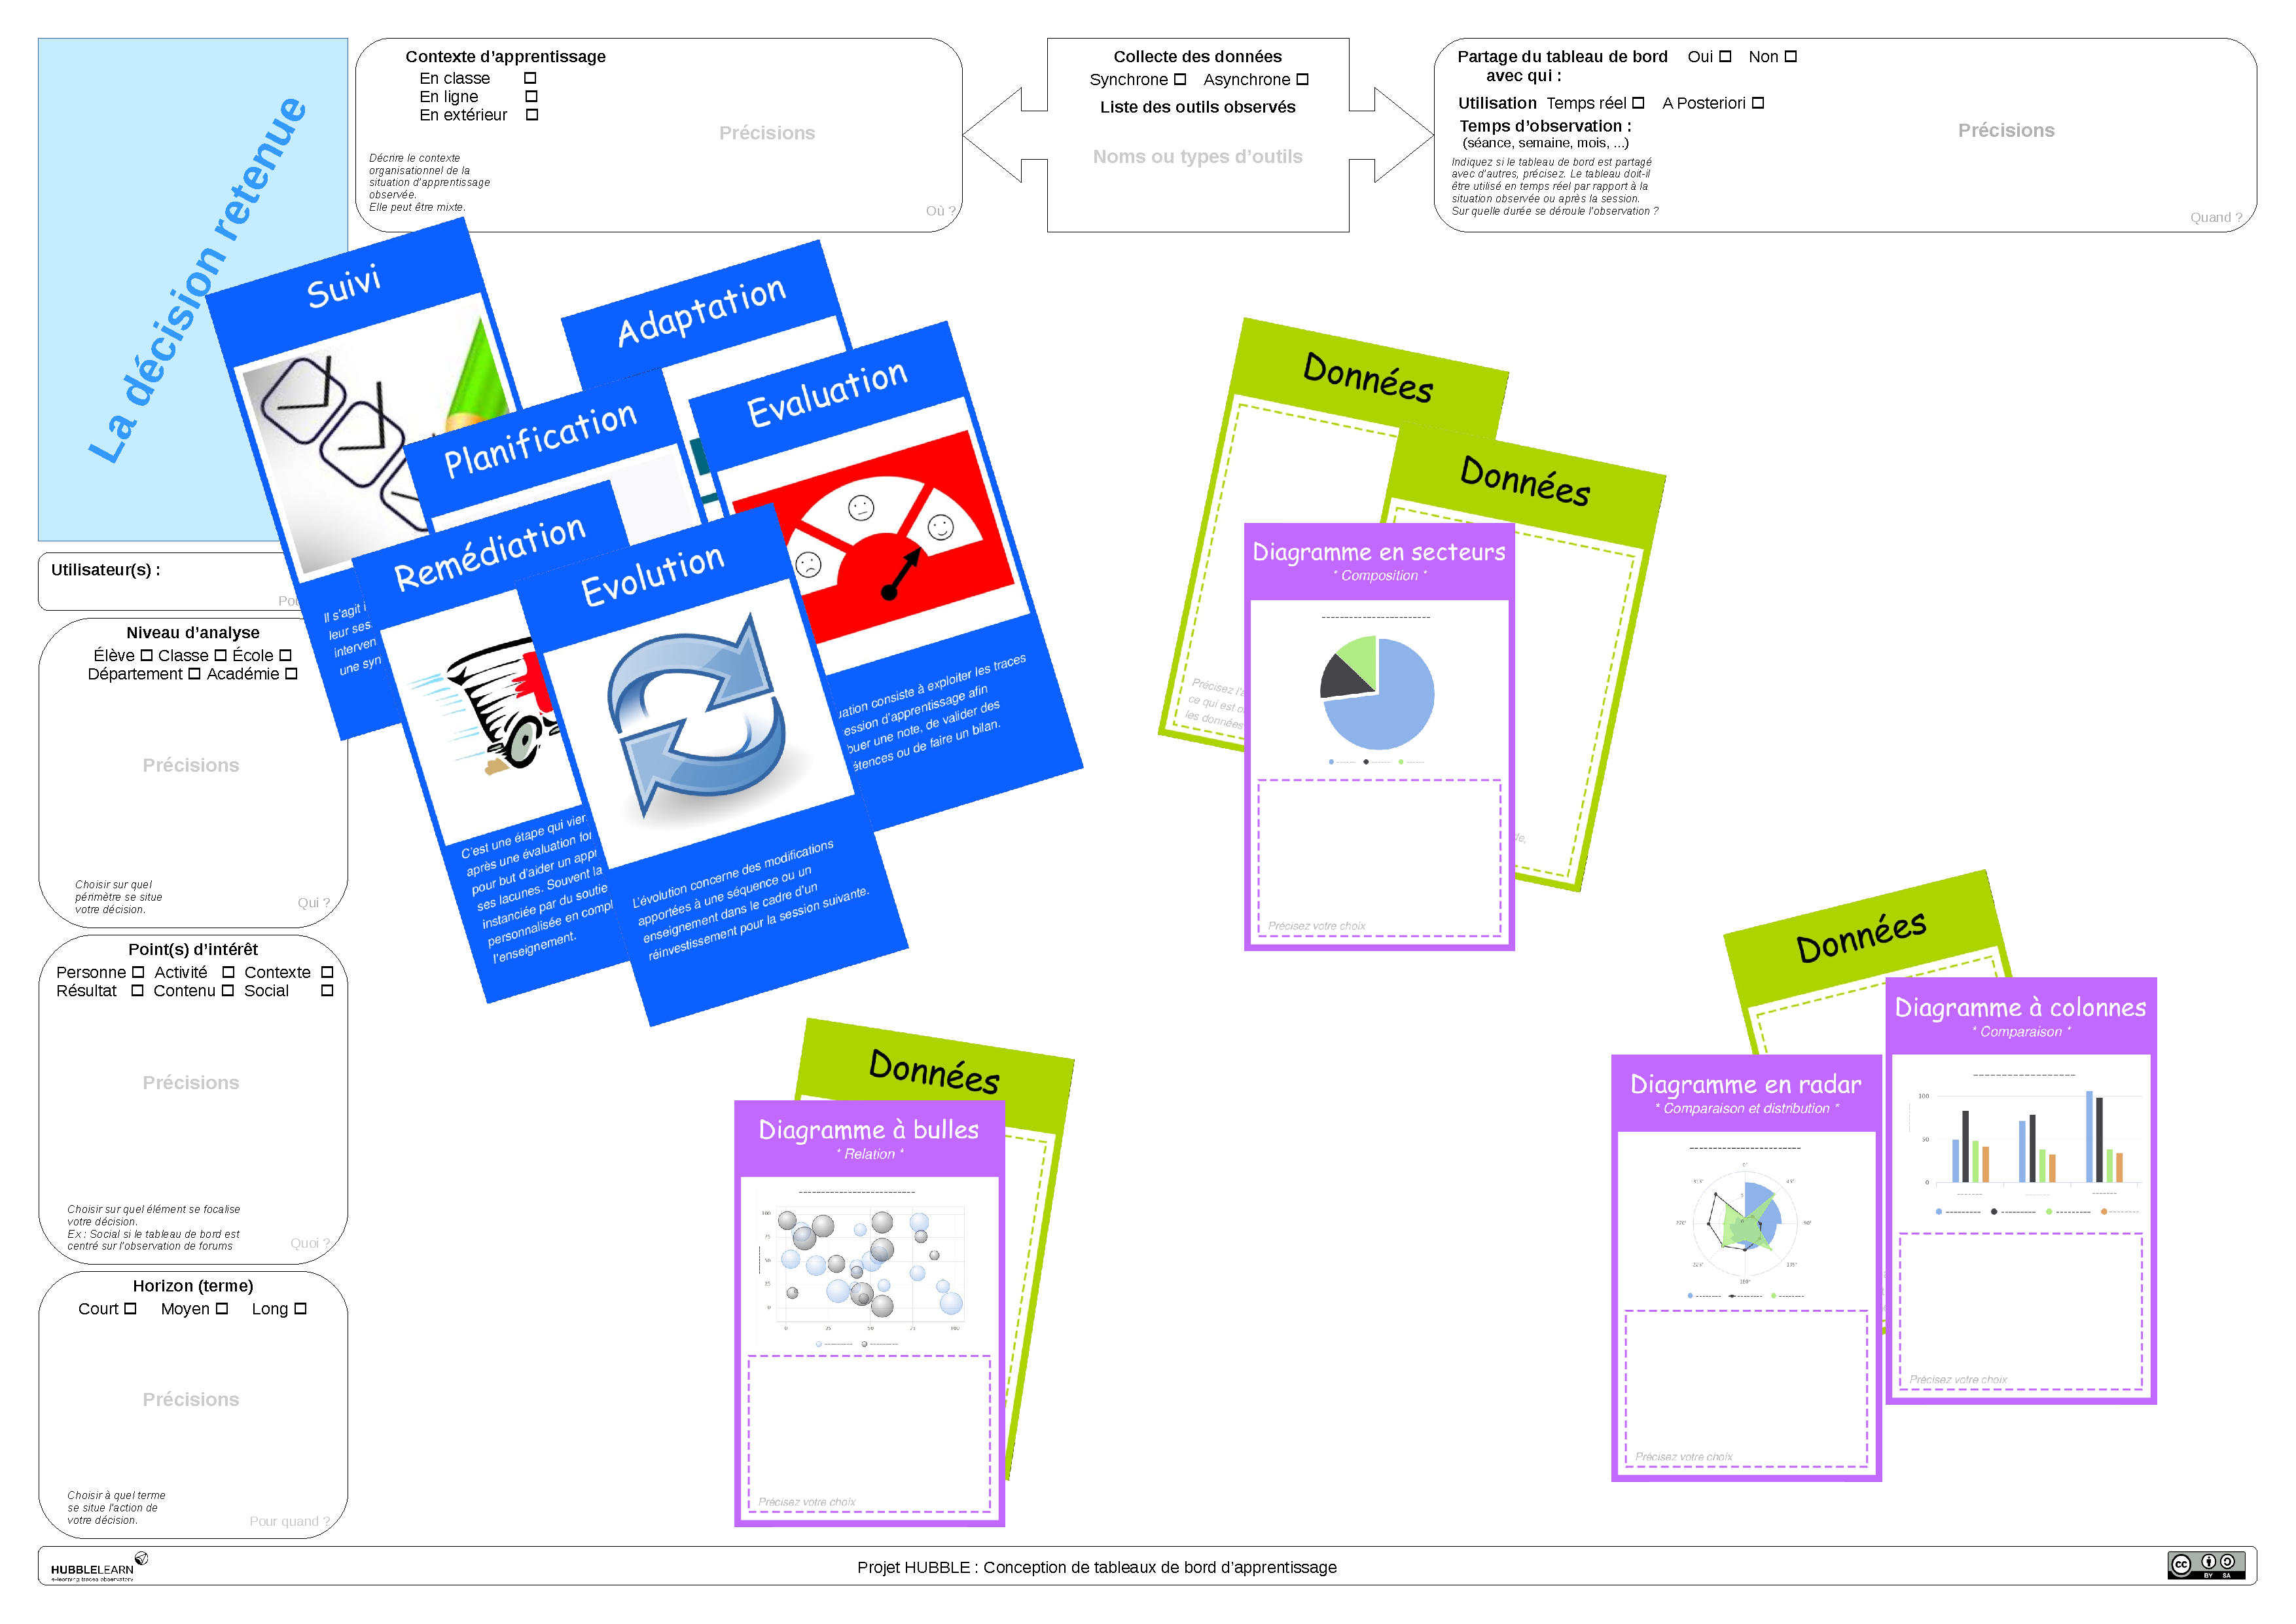
\includegraphics[width= \linewidth]{figs/plateau.pdf}
    \caption{Learning Dashboard Characterization Plateau}
    \label{fig:plateau}
    \end{figure}
First of all, as already mentioned, the central point of the dashboard from the users' point of view is the decision that is easier for them to express than the objective of observation.
We have therefore developed several so-called domain maps to identify the decision category (Remediation, Adaptation, Evolution, Evaluation, Monitoring, Planning), but also blank decision maps to let participants suggest other possibilities. These decision cards summarize on the back what the category means and on the front they provide space for participants to elaborate on their decision: Why do they need to make this decision? What
actions do they intend to implement? How does it fit into their pedagogy? These are the blue cards visible in the upper left corner of the characterization plateau in \ref{fig:plateau}.

On the characterization plateau, the location of the decision map is in the upper left corner so that participants collaborating on the plateau maintain a permanent view of this objective. This position was chosen to highlight the pivotal nature of this dimension. The plateau is then divided into different areas to specify the general context of the dashboard. A place is provided to precise the target user(s) of the dashboard. For each of the zones, the participants have the opportunity to provide details explaining their choices. The lists on the board are not fixed, participants can propose new values.

The purpose of this first plateau is to clarify what the dashboard is, its usefulness and its content. This is why we have left an important place on the plateau for the participants to design their content. They can use two types of cards: the measurement cards  and the visualization cards (respe. green and purple cards on figure \ref{fig:plateau}).
\begin{itemize}
    \item Measurement cards are blank cards in which it is necessary to describe the data that participants want to see in order to make their decision. They are asked to be accurate and to explain the data. For example, "I want to visualize learner engagement in the forum, so I need the number of messages posted and read per learner and per session". These measurement cards will then be associated with one or more visualization cards.
    \item Visualization cards depict different possibilities for graphically representing the data. For this purpose, participants are given a visual example of the representation, and are asked to indicate the title of their graph, the location of the data to be represented (for example, learners on the x-axis and the number of messages on the y-axis). They also have a space on the map to specify if needed their expectations from this visualization. To stimulate their creativity, we have designed blank visualization cards so that participants can propose their own graphical representation that they can easily understand.
\end{itemize}
Combining these two types of cards allows to associate elements of the "How" dimension with elements of the "What" dimension in a very flexible way.

For the prototyping, we invite the participants to think about to the formatting of their dashboards. For this, we offer several prototyping plateaus representing different equipment (web browser, smartphone, tablet). Participants are then asked to place the visualization cards from Step 1 in the locations they feel are most appropriate. They can also add artefacts describing the dashboard functionalities (button, refresh, title, scroll bar, menu, functions: filter, zoom, hide, print, save as image, etc.).

\subsection{User workshops}
In this section, we describe how to use our tool in a participatory workshop and then provide some initial feedback on its use.
\subsubsection{workshop setup}
A user workshop consists of 5 steps: introduction, dashboard characterization, dashboard prototyping, presentation, and summary. We adopt the basic process proposed by \citet*{lucero2016designing} and introduce a specific step for the layout of the dashboard.

\paragraph{Introduction}
The workshop starts with a presentation of the plateaux and maps (decision, measurement, visualization). Presentations are typically made by a facilitator whose task it is to lead the discussion. The maps can be presented either by the facilitator or by specialists in the field and/or in dashboard design. Participants are divided into teams of 2 to 6 people.
 
\paragraph{Dashboard characterization}
This step refers to the phase of co-creating and combining ideas. Participants are encouraged to specify their need through the first stage (see Figure 1) and the decision map. The discussion can be organized as they wish, but the goal is to fill in the different sections of the plateau. In addition, the participants can define the different measures they wish to have and associate visualization modes to these measures.
This combination step represents the crucial part of moving from the expression of the intended decision to the visualization objective. Having cards allows participants to associate several measures with a visualization and to combine several visualizations to make interaction with the measures tangible. In this phase, the facilitator plays an important role in encouraging participants to explore other combinations and to formalize their ideas to the best of their ability. Participants can write on the plateau their explanations or the justification of their choices, which will help in the creation of the dashboard. The result of this step is twofold : (i) a shared and clear understanding of the needs (ii) a collection of the needs of the dashboard.

\paragraph{Dashboard prototyping}
This step is intended for the visual representation of the dashboard, both at the organization and visualization level as well as at the interaction level, using the trays representing a selected piece of equipment. The support provided by a dashboard designer can motivate the participants to develop their projection in this future tool intended for them. This step concludes the phase of convergence towards the expressed need. The result of this step is a first hardcopy prototype established by the participants.

\paragraph{Representation}
After the two creation steps, the participants are asked to take the time to consolidate their results and the concepts they have chosen. If several groups are present, the different groups can do a cross-referenced restitution. This step allows a pooling of proposals.

\paragraph{Sumarry}
After the workshop, the proposed new maps and dashboards are collected with three complementary objectives: production, capitalization and evaluation.
\begin{itemize}
    \item \textit{Production.} This collection allows, through the dashboard generation process, to produce a dashboard matching the expressed needs.
    \item \textit{Capitalization.} Capitalization covers all the elements proposed during the workshop, to feed the Hubble project's study base in general and the base used to generate learning dashboards in particular. New maps may be produced to complete the tool presented here.
    \item \textit{Evaluation.} Evaluation of the tool and the workshop process are ensured for improvement.
\end{itemize}


\subsubsection{Initial user feedback}
This participatory design tool has been tested in two different contexts. A first test workshop was set up with teachers in computer science OTCs; a presentation and test workshop was proposed during national meetings between researchers and national education supervisory staff. During each of these tests, the conduct of the workshop was observed and filmed, with the agreement of the participants. A satisfaction questionnaire was also used to gather participants' opinions.

\subsubsection{Workshop with computer scientists}
This first test in an educational context was carried out with two test groups of 4 and 2 teachers in the DUT Informatique. The first group (G1) consisted of a teacher in charge of the pedagogical situation to be observed and 3 colleagues wishing to collaborate on the design of his dashboard. The second group (G2) has a different profile as it consists of 2 teachers involved in the same learning situation with the same students. 

Both groups started in the same way to analyze the decision cards in order to select the most appropriate one. The first group came up with several possible decisions and focused on the evaluation as it seemed like a map with a wider scope. The second group went directly to the decision related to monitoring as theu were in a tutored project situation with a necessary follow-up for supervision. 

Secondly, the two groups took different paths in the conception phase. Group G1 exploited the maps and annotated them. They made numerous hypotheses and produced many data maps, not knowing if all of them would be useful in the end. Group G2 started by thinking about the tool needed for the students to express their progress through the different phases of the project, which is the same as describing the data they need, but they did not use any maps. In the end, they constructed a data grid. 

\begin{figure}[!htp]
    \centering
    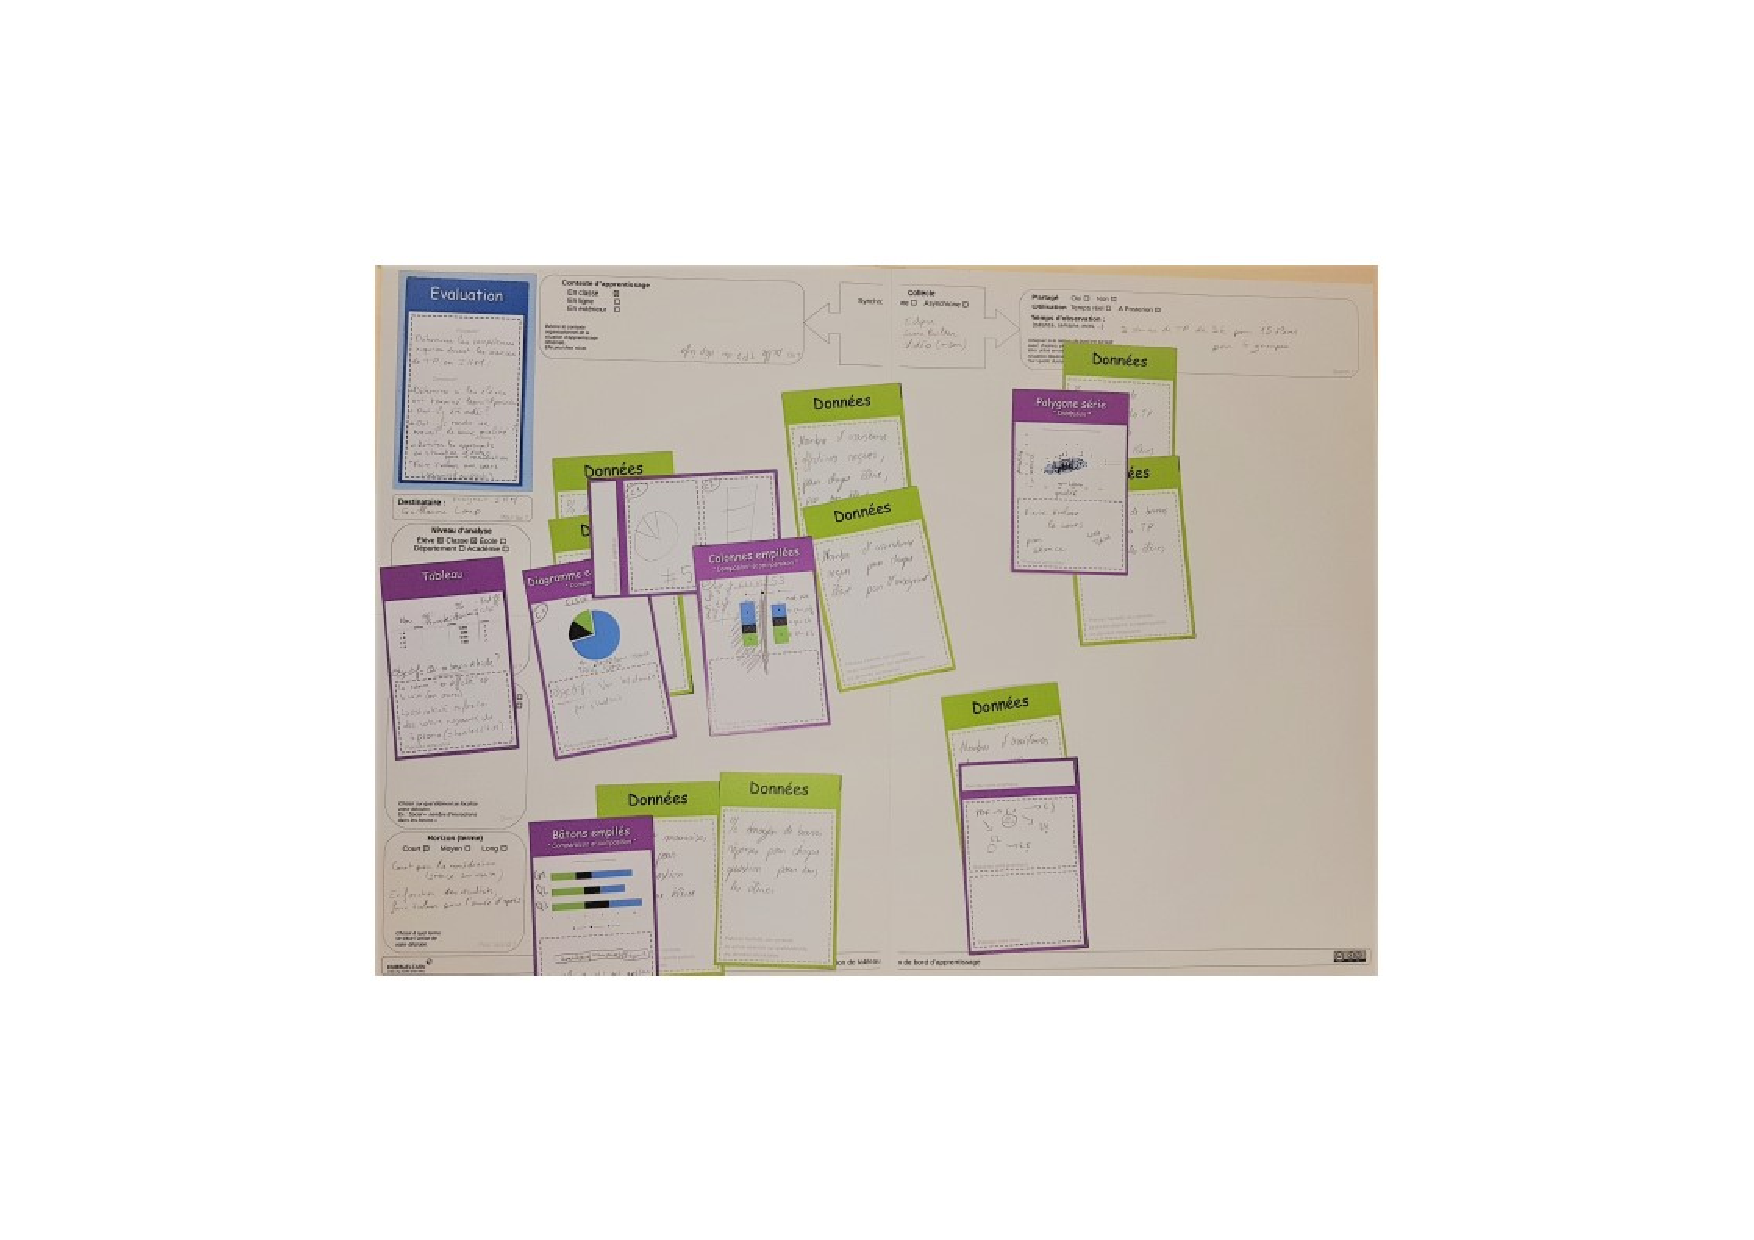
\includegraphics[width= \linewidth]{figs/fig2.pdf}
    \caption{A characterization plateau at the end of the first user workshop}
    \label{fig:fig2}
    \end{figure}

    Also, in terms of graphical representation, the G1 group made good use of the maps (see Figure \ref{fig:fig2}). They filtered their dataset to keep only the main points and realized that there were clearly two sets of information corresponding to two types of decisions: remediation and evolution. They therefore reconsidered their first choice of decision. Group G2 took inspiration from the visualization maps to develop a new type of graphical representation corresponding to a composition of several maps. They then drew the graphic representation they needed.

Finally, on the section related to the design of the dashboard interface, the G2 group was satisfied with its summary graph for monitoring, while the G1 group imagined 2 different and disconnected interfaces, which reflects the fact that decision is a central point and that clarifying it allows participants to organize the dashboard in a different way. 

Both groups agree that the proposed materials are pleasant to use, encourage and energize the exchange. The two groups had very different experiences with lively debates, which confirms the quality of the support for creativity. The choice to highlight the decision objective of the dashboard as a pivotal element of the design was effective in allowing participants to focus on an explicit need.

Comparing with the workshops held previously, especially the workshop with Tactileo Map teachers, we notice a saving of time, a better productivity and an intensification of exchanges. Indeed, during our first study, we had grouped the teachers in teams of two and we had to play an important role as facilitators. We had to question the teachers and push them to think. This took them out of their comfort zone and produced interesting results, but the full-day session was challenging. Thanks to our design spaces, this new session was reduced to two and a half hours, the exchanges were more natural and our role was reduced to observation as well as answering a few comprehension questions. Moreover, during the first session, we had only obtained a description of the learning situation, a list of data and some means of representation. In this workshop, we also obtained the information related to the decision as well as the dashboard interface mock-ups corresponding to what teachers needed (see Figure \ref{fig:fig3}).
\begin{figure}[!htp]
    \centering
    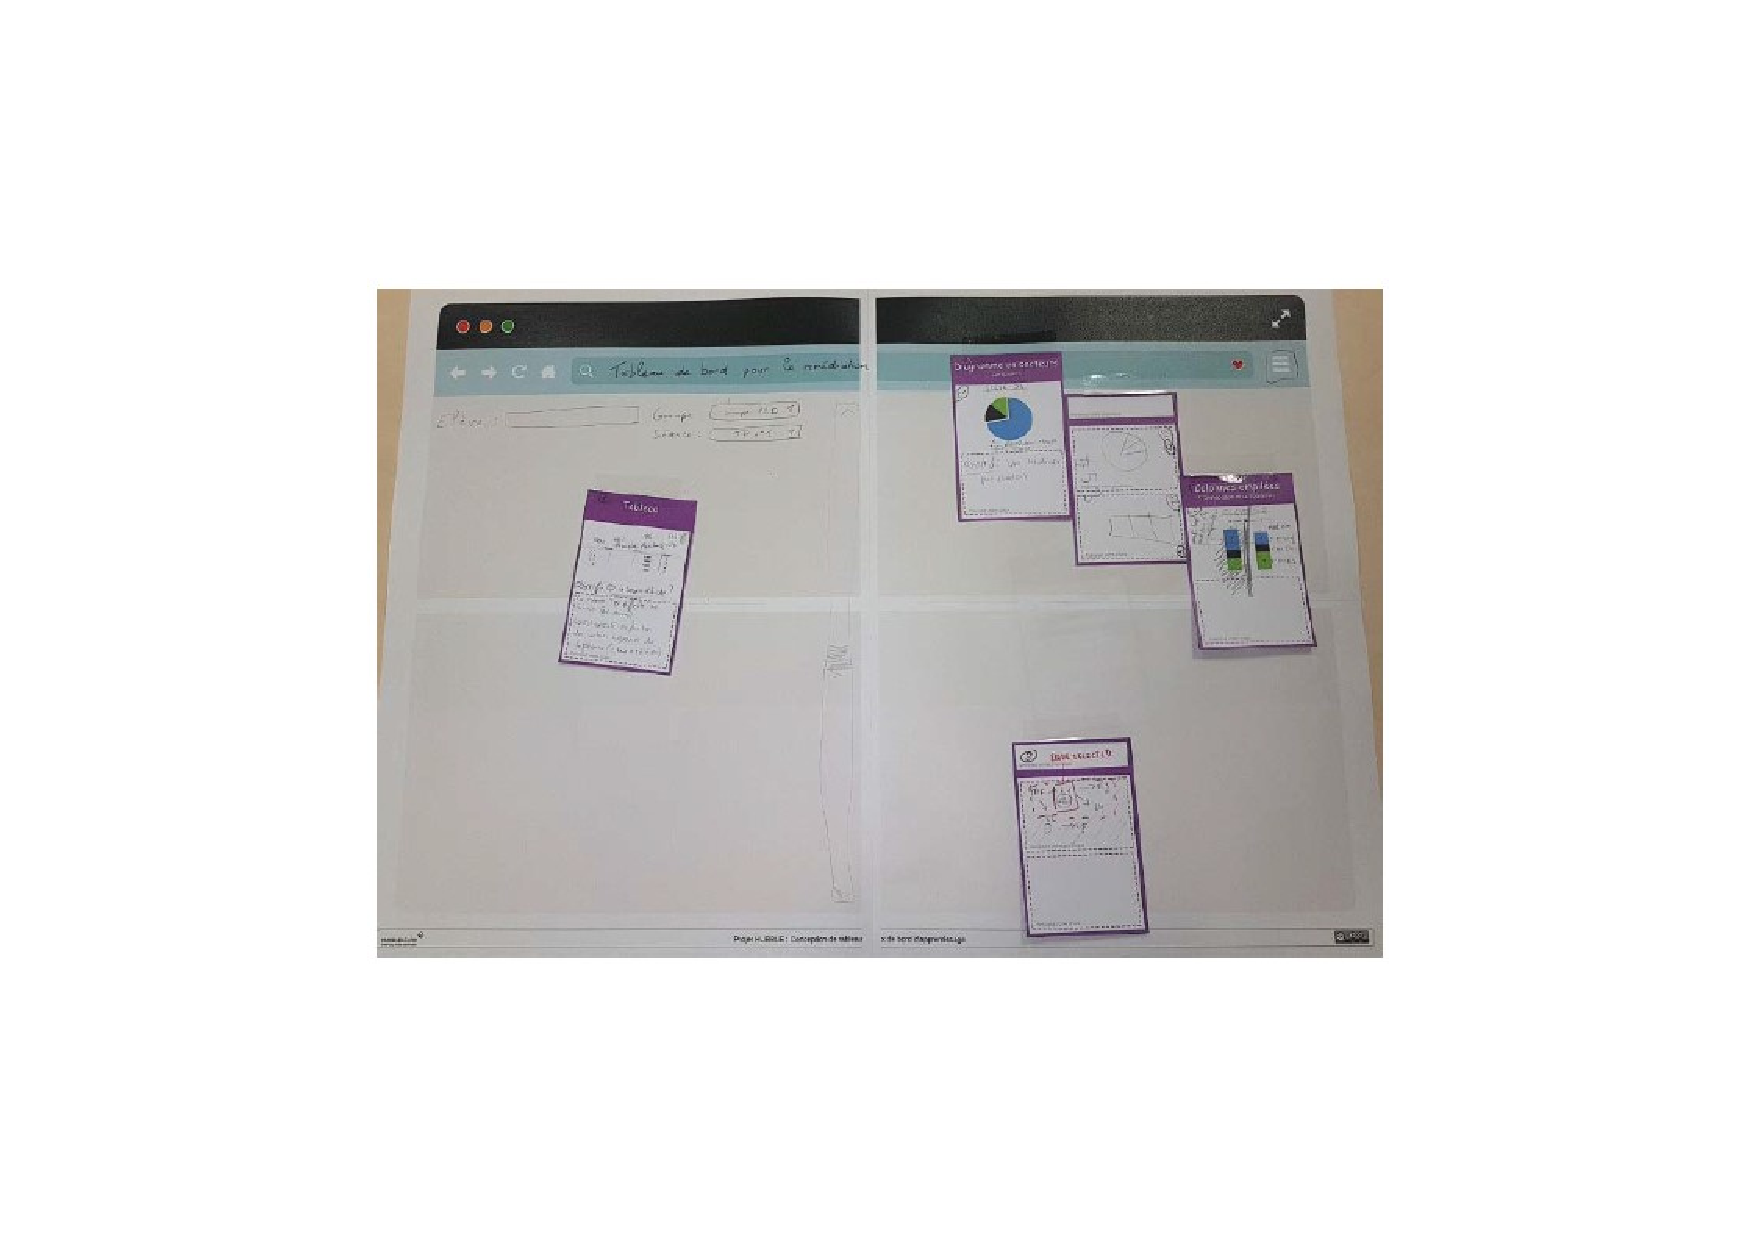
\includegraphics[width= \linewidth]{figs/fig3.pdf}
    \caption{An example of a prototyping plateau at the end of the first user workshop}
    \label{fig:fig3}
    \end{figure}
\subsubsection{Presentation workshop for national education inspectors}
This workshop made it possible to constitute two groups of four and three participants respectively. In both groups, a great dynamic of exchanges was set up, and the participants were able to test and discuss many options on the different dimensions of the design space. Compared to the previous workshop, we observed two other modes of progress, which seems to confirm that the proposed tool does not restrict the flow of exchanges. Both groups actually propose dashboards corresponding to a need identified in a limited time. 

\subsubsection{Questionnaire results}
The size of the group does not allow for a statistical analysis of our questionnaire. This questionnaire includes seven questions asking for a level of agreement on a Lickert scale with 5 levels. Two questions deal with the handling of the tool ( plateaux and maps), three questions on the quality of the resulting solution (precision, originality, relevance) and two on group work (dynamics, convergence). Two open-ended questions allow the participants to express their opinion. Overall, the level of satisfaction seems high (no answer below 3), with a majority of answers at level 4 or 5. Among these, the question "The plateaux and the cards helped to create a good group dynamic" received the best result with a response rate at level 5 of more than 75\%.

\subsubsection{Future test}
Following the workshop with the national education inspectors, a kit with our material is  available in the Productions section of the Hubble project website.


\section{Conclusion}
Drawing inspiration from participatory design approaches used in game design \cite{hallifax2018design} or in entrepreneurship \cite{osterwalder2010business}, we propose in this article a design space through a support tool for the participatory design of learning dashboards, and its implementation in the framework of participatory workshops. This tool combines a board and maps supporting both decision support and the provision of design alternatives. It meets the dual objective of expressing user needs and capitalizing on these needs and the corresponding dashboards. 

The initial feedback from a test workshop is encouraging, and shows that this type of workshop effectively facilitates cooperation and further exploration of alternatives. According to \citet{mackay1997radicalement} and \citet{knibbe2016}, participation in such workshops can also contribute to developing the appropriation of such tools by the participants. This hypothesis seems particularly interesting in the context of Learning Analytics in which potential users often lack maturity in the use of such digital devices, whereas relevant feedback is a source of appropriation of digital practices.

\bibliographystyle{ACM-Reference-Format}
\bibliography{references}



\end{document}
\endinput